\section{System structure}

\begin{figure}\label{fig:system_architecture}
  \caption{System architecture of the proposed MIMO WIPT system \cite{Ma2019}}
  \centering
    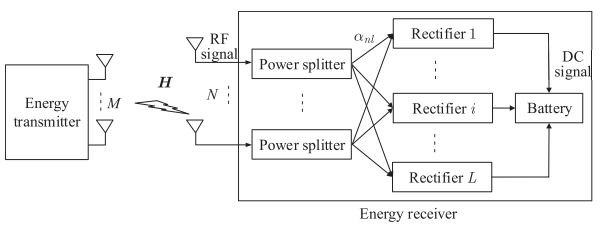
\includegraphics[width=0.5\textwidth]{system_architecture}
\end{figure}

We consider a point-to-point MIMO WIPT system with $M$ transmitters, $N$ receivers and $L$ rectifiers. Figure \ref{fig:system_architecture} illustrates the system structure \textit{from energy perspective}. In the proposed design, each receive antenna is followed by a splitter that determines the input power to the rectifiers. Specifically, when the received power level is relatively low, the splitters will combine all energy branches in one rectifier to enjoy the benefit of harvester nonlinearity. In contrast, when the power is sufficiently high, the components will be equally divided to rectifiers to avoid the low conversion efficiency of diode breakdown region \cite{Clerckx2019}. The harvested power is then combined and stored in the battery.


\section{Non-linear Energy Harvester Model}

A nonlinear EH model proposed in \cite{Boshkovska2015} whose parameters relies on curve fitting will be compared with the diode nonlinear model designed by \cite{Clerckx2018}.


\section{Waveform Design and Transceiver Architecture}

\begin{figure}\label{fig:transmitter}
  \caption{Dual-mode SWIPT transmitter \cite{Park2018}}
  \centering
    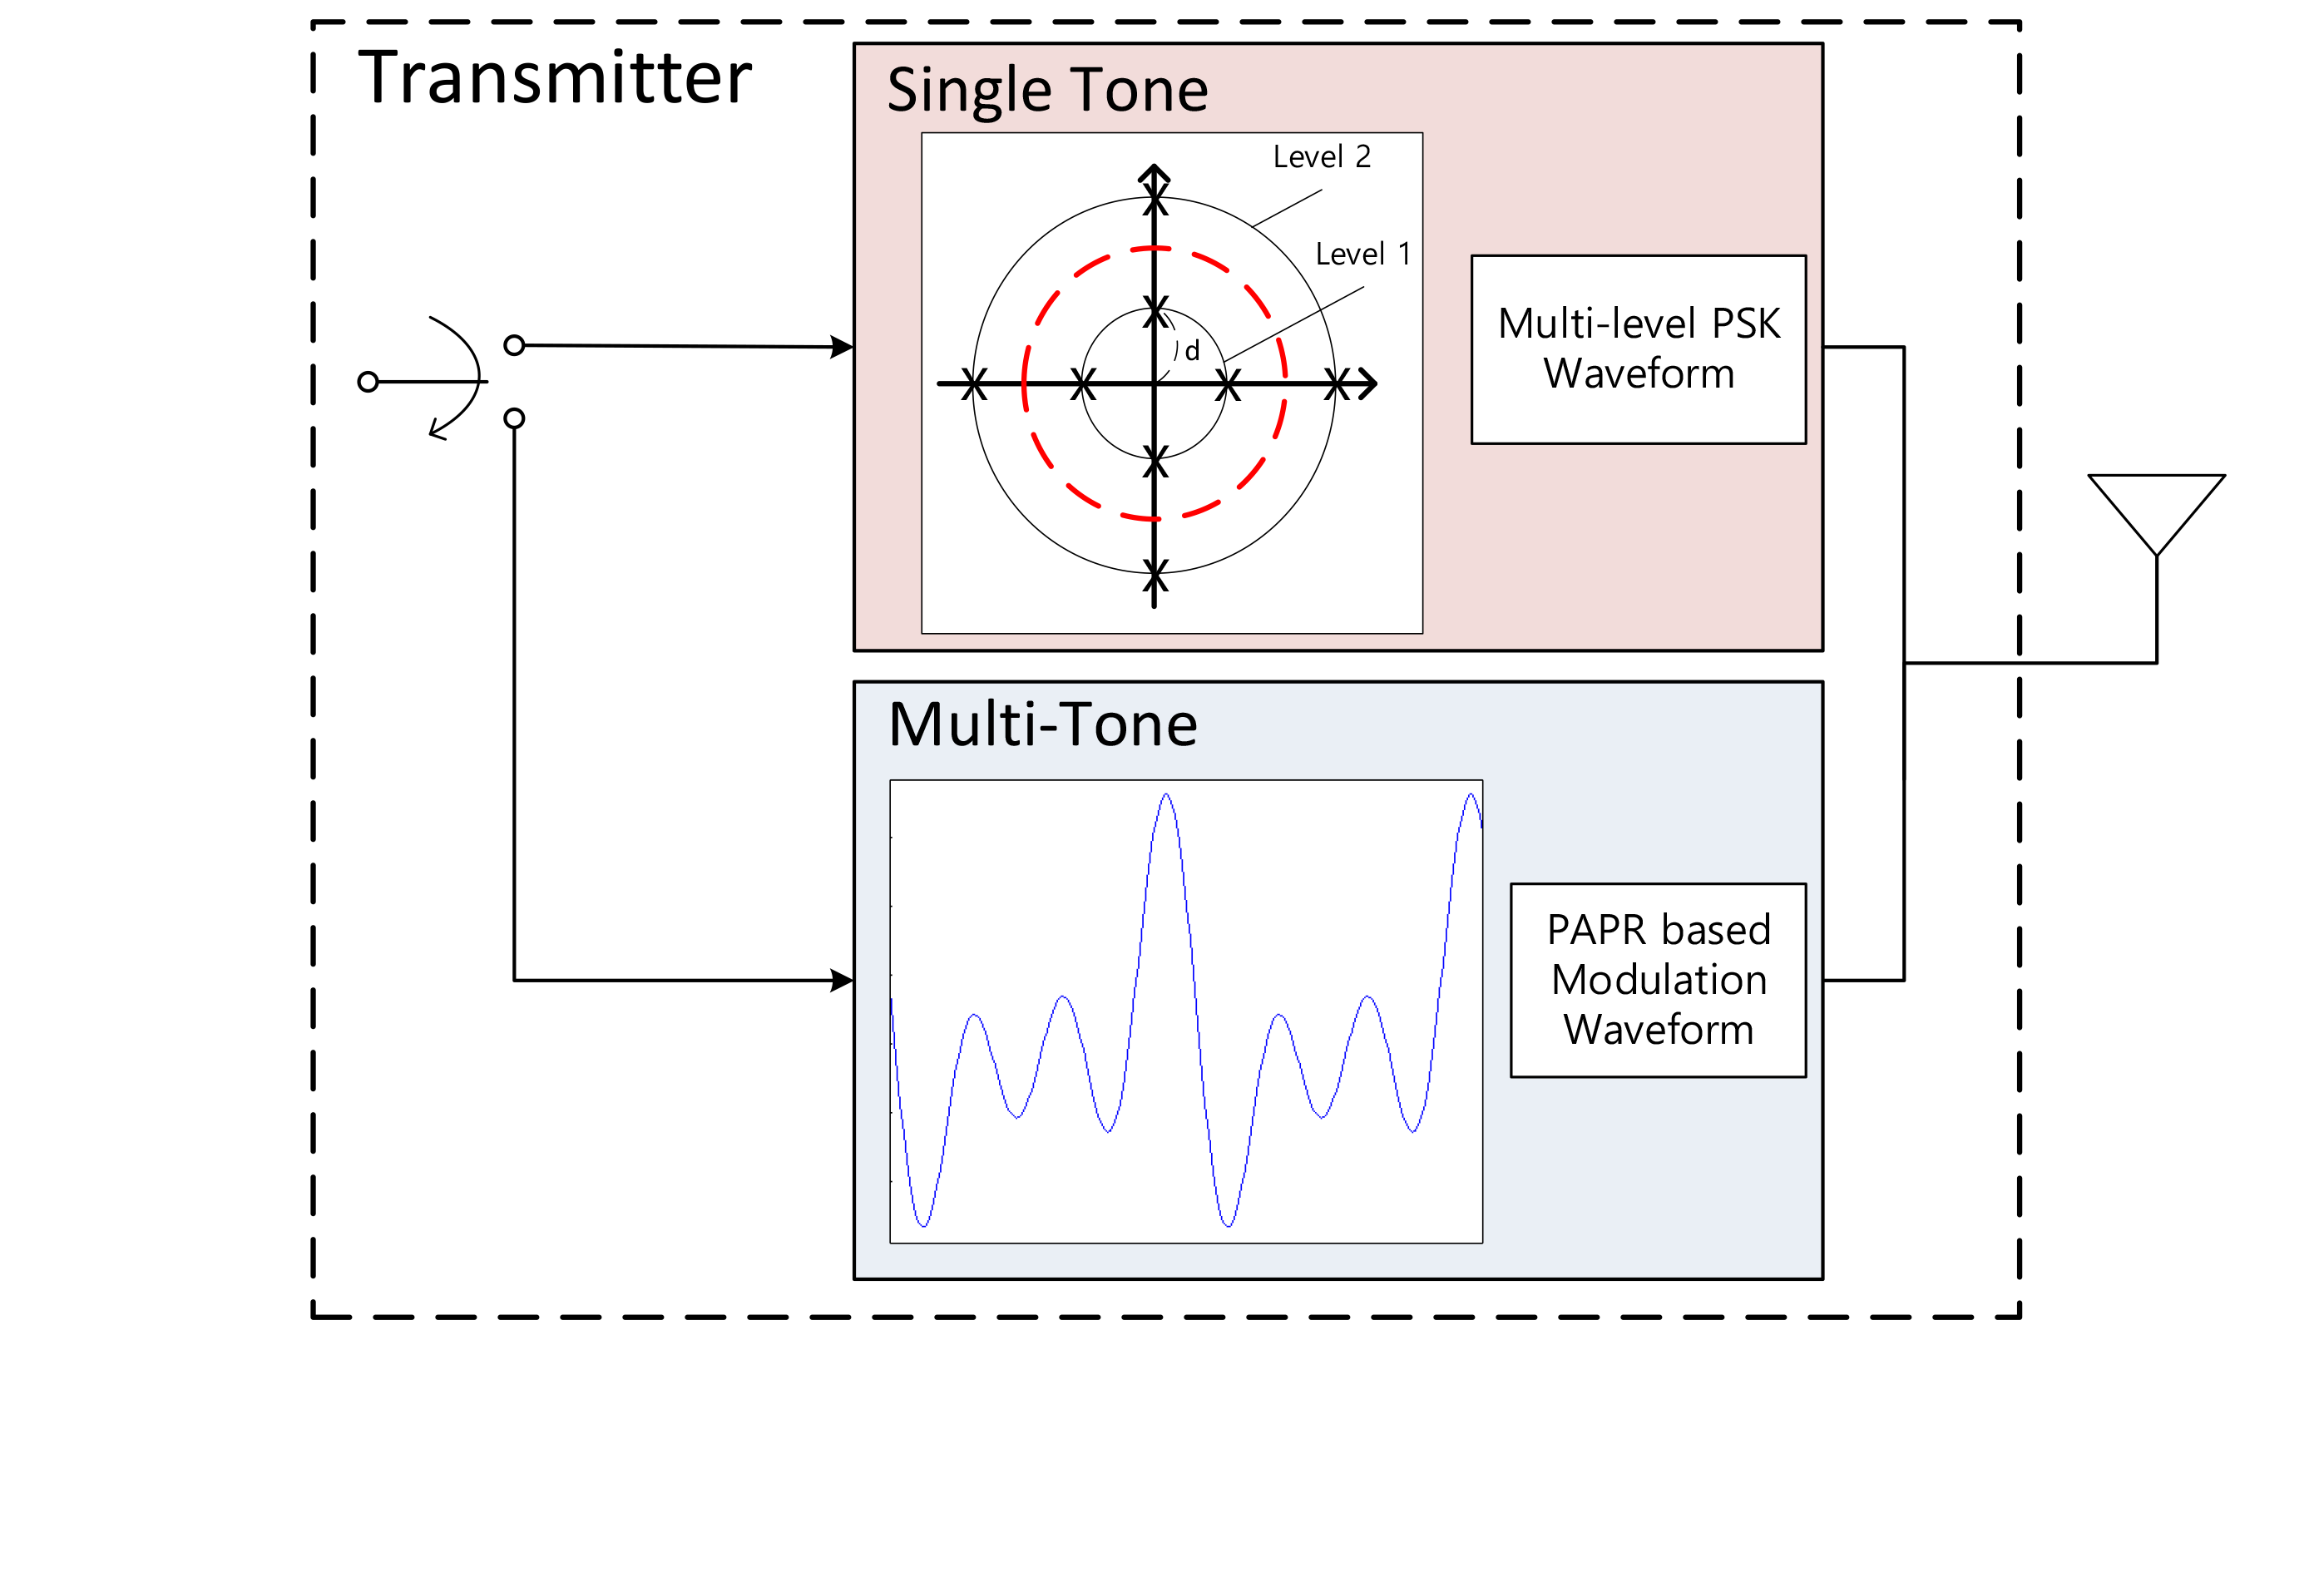
\includegraphics[width=0.5\textwidth]{transmitter}
\end{figure}

As shown in Figure \ref{fig:transmitter}, each transmitter consists of a single-tone and a multi-tone signal generator. We will design an adaptive MS algorithm to control the transmission mode according to the received power. The single-tone waveform modulates the amplitude and the phase simultaneously and is suitable for high rate transmission. In contrast, the multi-tone waveform encodes the information by choosing a combination of tones with a specific PAPR level. Therefore, $Q$ tones can be used to transmit $\log { & _2}Q$ bits by uniquely mapping to subsets. Compared with conventional techniques, the tone-index multisine modulation increases the operation range, boosts the harvested power, and reduce the complexity in modulation and demodulation. Interestingly, it requires a dynamic design to find the tones experiencing better channel gains and assign the subsets correspondingly, especially for FS channels.

\begin{figure}\label{fig:receiver}
  \caption{Dual-mode SWIPT transmitter \cite{Park2018}}
  \centering
    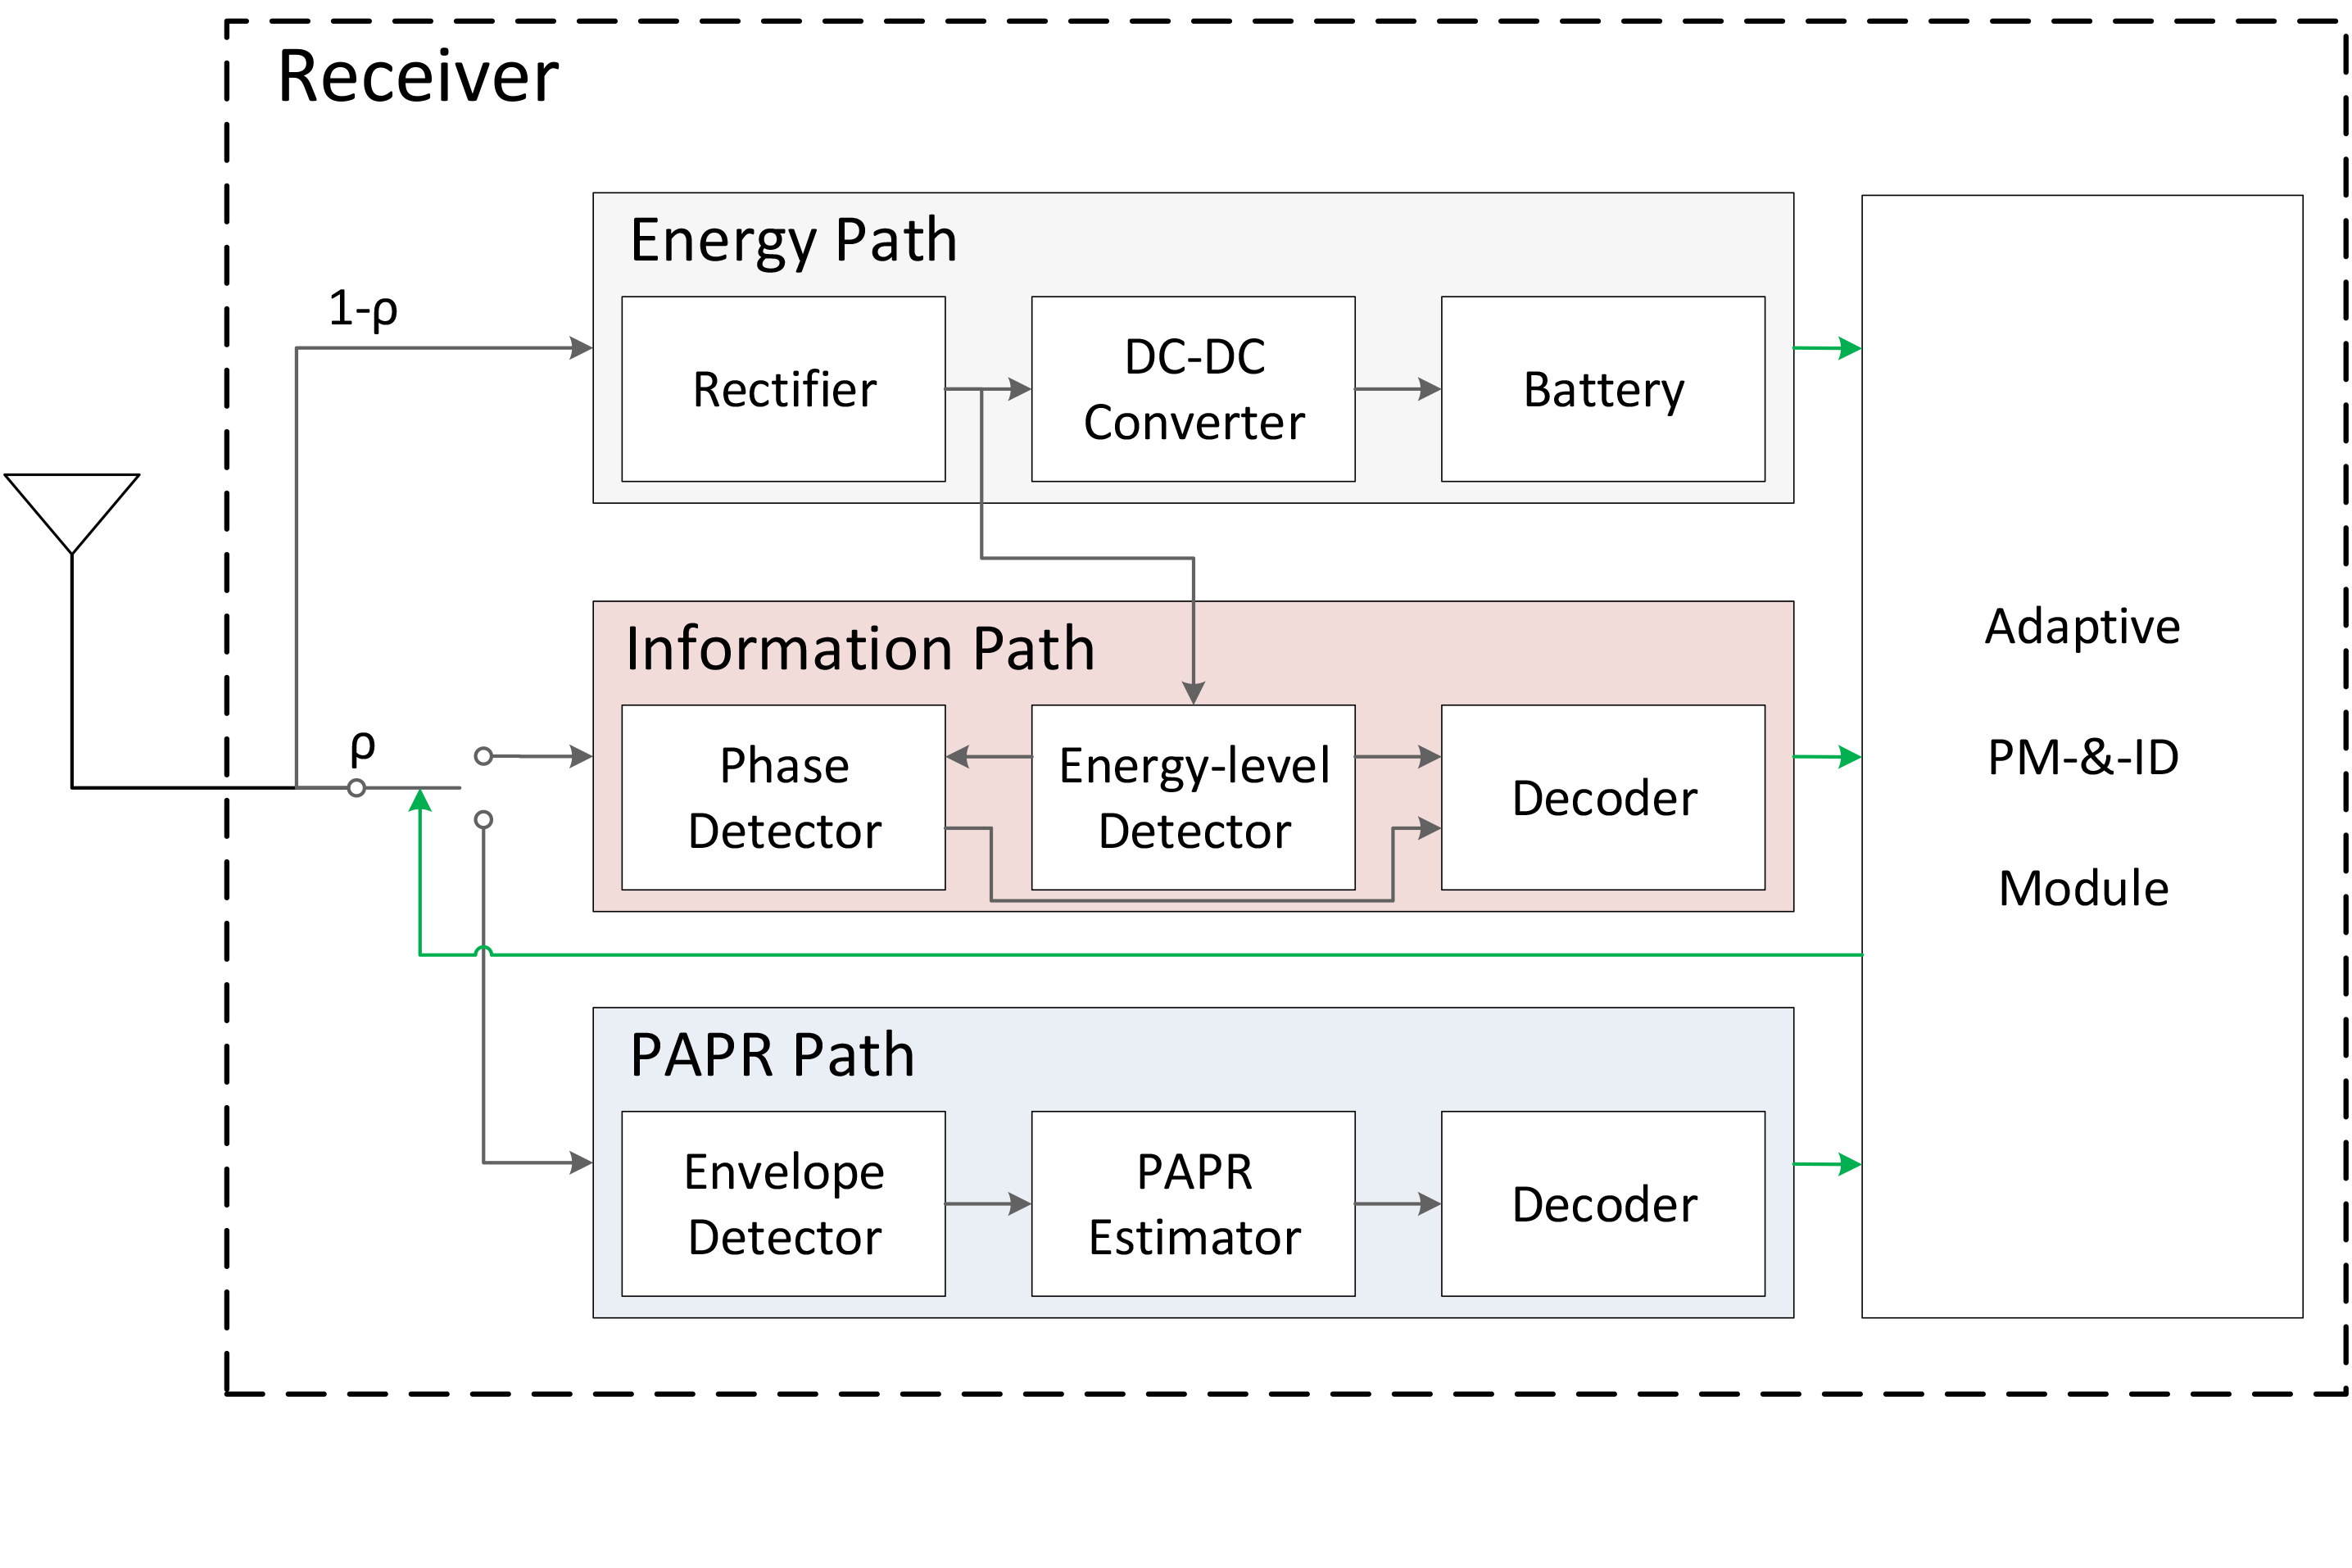
\includegraphics[width=0.5\textwidth]{receiver}
\end{figure}

The block diagram of a integrated receiver is shown in Figure \ref{fig:receiver}. Note that there are multiple receiver for the MIMO case, and for the energy paths we introduce power splitters before the rectifier cluster. With power-information ratio $\rho $, the received signal is divided into energy stream (goes through energy path) and information stream (single-tone goes through information path, multi-tone goes through PAPR path). Note that this ratio is different from the power splitting ratios which are used to reallocate power to rectifiers. It is argued in \cite{Park2018} that an infinitesimally small $\rho $ is enough for ID for the property of integrated receiver \cite{Zhou2013}, and most of the received signal can be used for EH. Energy path is used for both power collection and energy-level information decoding. It not only transmits the amplitude to information path but also provides the power for demodulation. The remaining power will be stored in the battery. Information path estimates CSI then decodes the phase information accordingly. In comparison, PAPR path decodes the envelope-based information by measuring the PAPR of the received signal. It does not require channel estimation and active devices, therefore the power consumption is significantly less than information path.

